%%%% Proceedings format for most of ACM conferences (with the exceptions listed below) and all ICPS volumes.
\documentclass[sigconf]{acmart}
%%%% As of March 2017, [siggraph] is no longer used. Please use sigconf (above) for SIGGRAPH conferences.

%%%% Proceedings format for SIGPLAN conferences 
% \documentclass[sigplan, anonymous, review]{acmart}

%%%% Proceedings format for SIGCHI conferences
% \documentclass[sigchi, review]{acmart}

%%%% To use the SIGCHI extended abstract template, please visit
% https://www.overleaf.com/read/zzzfqvkmrfzn

\usepackage{booktabs} % For formal tables
\usepackage{bm}
\usepackage{amsmath}
\usepackage{algorithm}
\usepackage{indentfirst}
% \usepackage{algorithmic}
\usepackage[noend]{algpseudocode}
\usepackage{multirow}

% Copyright
%\setcopyright{none}
%\setcopyright{acmcopyright}
%\setcopyright{acmlicensed}
\setcopyright{rightsretained}
%\setcopyright{usgov}
%\setcopyright{usgovmixed}
%\setcopyright{cagov}
%\setcopyright{cagovmixed}


% DOI
\acmDOI{10.475/123_4}

% ISBN
\acmISBN{123-4567-24-567/08/06}

%Conference
%Comm
% \acmConference[WOODSTOCK'97]{ACM Woodstock conference}{July 1997}{El
%   Paso, Texas USA} 
% \acmYear{1997}
% \copyrightyear{2016}

% \acmPrice{15.00}
%Comm


\begin{document}
\title{Efficient Multistream Regression}
\titlenote{Produces the permission block, and
  copyright information}
% \subtitle{Extended Abstract} %Comm
% \subtitlenote{The full version of the author's guide is available as
%   \texttt{acmart.pdf} document} %Comm


\author{Ahsanul Haque}
% \authornote{Dr.~Trovato insisted his name be first.} %Comm
\orcid{1234-5678-9012}
\affiliation{%
  \institution{The University of Texas at Dallas}
  \streetaddress{800 W Campbell Rd} 
  \city{Richardson} 
  \state{Texas} 
  \postcode{75083-0688}
}
\email{Ahsanul.Haque@utdallas.edu}

\author{Bo Dong}
% \authornote{The secretary disavows any knowledge of this author's actions.} %Comm
\affiliation{%
  \institution{The University of Texas at Dallas}
  \streetaddress{800 W Campbell Rd} 
  \city{Richardson} 
  \state{Texas} 
  \postcode{75083-0688}
}
\email{bxd130630@utdallas.edu}

\author{Yifan Li}
% \authornote{The secretary disavows any knowledge of this author's actions.} %Comm
\affiliation{%
  \institution{The University of Texas at Dallas}
  \streetaddress{800 W Campbell Rd} 
  \city{Richardson} 
  \state{Texas} 
  \postcode{75083-0688}
}
\email{yli@utdallas.edu}

\author{Yang Gao}
% \authornote{The secretary disavows any knowledge of this author's actions.} %Comm
\affiliation{%
  \institution{The University of Texas at Dallas}
  \streetaddress{800 W Campbell Rd} 
  \city{Richardson} 
  \state{Texas} 
  \postcode{75083-0688}
}
\email{yxg122530@utdallas.edu}

\author{Latifur Khan}
% \authornote{The secretary disavows any knowledge of this author's actions.} %Comm
\affiliation{%
  \institution{The University of Texas at Dallas}
  \streetaddress{800 W Campbell Rd} 
  \city{Richardson} 
  \state{Texas} 
  \postcode{75083-0688}
}
\email{lkhan@utdallas.edu}

% Comm
% \author{Charles Palmer}
% \affiliation{%
%   \institution{Palmer Research Laboratories}
%   \streetaddress{8600 Datapoint Drive}
%   \city{San Antonio}
%   \state{Texas} 
%   \postcode{78229}}
% \email{cpalmer@prl.com}

% \author{John Smith}
% \affiliation{\institution{The Th{\o}rv{\"a}ld Group}}
% \email{jsmith@affiliation.org}

% \author{Julius P.~Kumquat}
% \affiliation{\institution{The Kumquat Consortium}}
% \email{jpkumquat@consortium.net}
% Comm

% The default list of authors is too long for headers}
% \renewcommand{\shortauthors}{B. Trovato et al.}


\begin{abstract}
In a data stream regression problem, the predicted values of data instances are generated from a non-stationary process. According to past studies, scholars were focusing on problems under different scenarios such as covariant shift or concept drift. However, lots of these theories are discussing one scenario while keeping others consistent. For example, the training and testing data distribution are assumed to be similar, and true output value related to stream instances would be available. However, in practice these assumptions are not always valid. In lots of stream regression problems, only a fraction of values may be available soon after the prediction. If we use only this small fraction of data to train the model, sampling bias, or shift of the input distribution could be introduced accordingly. Thus the prediction generated by this data sample would not be accurate. Therefore how to appropriately handling this issue is a challenge. Moreover, if the conditional probability between the training data sample and testing data sample differs under a data stream setting, more estimation biases will be introduced as well. 

In this paper, we present a setting of multistream regression problem, involving two independent non-stationary data generating process. A source stream continuously generates data instances with values of output while the target stream generates data instances without values of output. Notice here the distribution of instances may vary. Hence the issue we want to address here, which is called Multistream Regression, is to estimate the output of each instance in target stream, while using output available on the source stream. Since the concept drift may occur between these two streams, a concept drift detection framework is designed and implemented. An assemble model is built to update the model built before the concept drift point in the source stream. Then we evaluate the multistream regression's performance on synthetic data sets.\footnote{This is an abstract footnote}
\end{abstract}

%
% The code below should be generated by the tool at
% http://dl.acm.org/ccs.cfm
% Please copy and paste the code instead of the example below. 
%


\begin{CCSXML}
<ccs2012>
 <concept>
  <concept_id>10010520.10010553.10010562</concept_id>
  <concept_desc>Computer systems organization~Embedded systems</concept_desc>
  <concept_significance>500</concept_significance>
 </concept>
 <concept>
  <concept_id>10010520.10010575.10010755</concept_id>
  <concept_desc>Computer systems organization~Redundancy</concept_desc>
  <concept_significance>300</concept_significance>
 </concept>
 <concept>
  <concept_id>10010520.10010553.10010554</concept_id>
  <concept_desc>Computer systems organization~Robotics</concept_desc>
  <concept_significance>100</concept_significance>
 </concept>
 <concept>
  <concept_id>10003033.10003083.10003095</concept_id>
  <concept_desc>Networks~Network reliability</concept_desc>
  <concept_significance>100</concept_significance>
 </concept>
</ccs2012>  
\end{CCSXML}

% Comm
% \ccsdesc[500]{Computer systems organization~Embedded systems}
% \ccsdesc[300]{Computer systems organization~Redundancy}
% \ccsdesc{Computer systems organization~Robotics}
% \ccsdesc[100]{Networks~Network reliability}
% Comm

% We no longer use \terms command
%\terms{Theory}

\keywords{Regression, Covariate Shift, Concept Drift, Data Stream}

%% Used in some conference proceedings e.g. sigplan and sigchi
% \begin{teaserfigure}
%   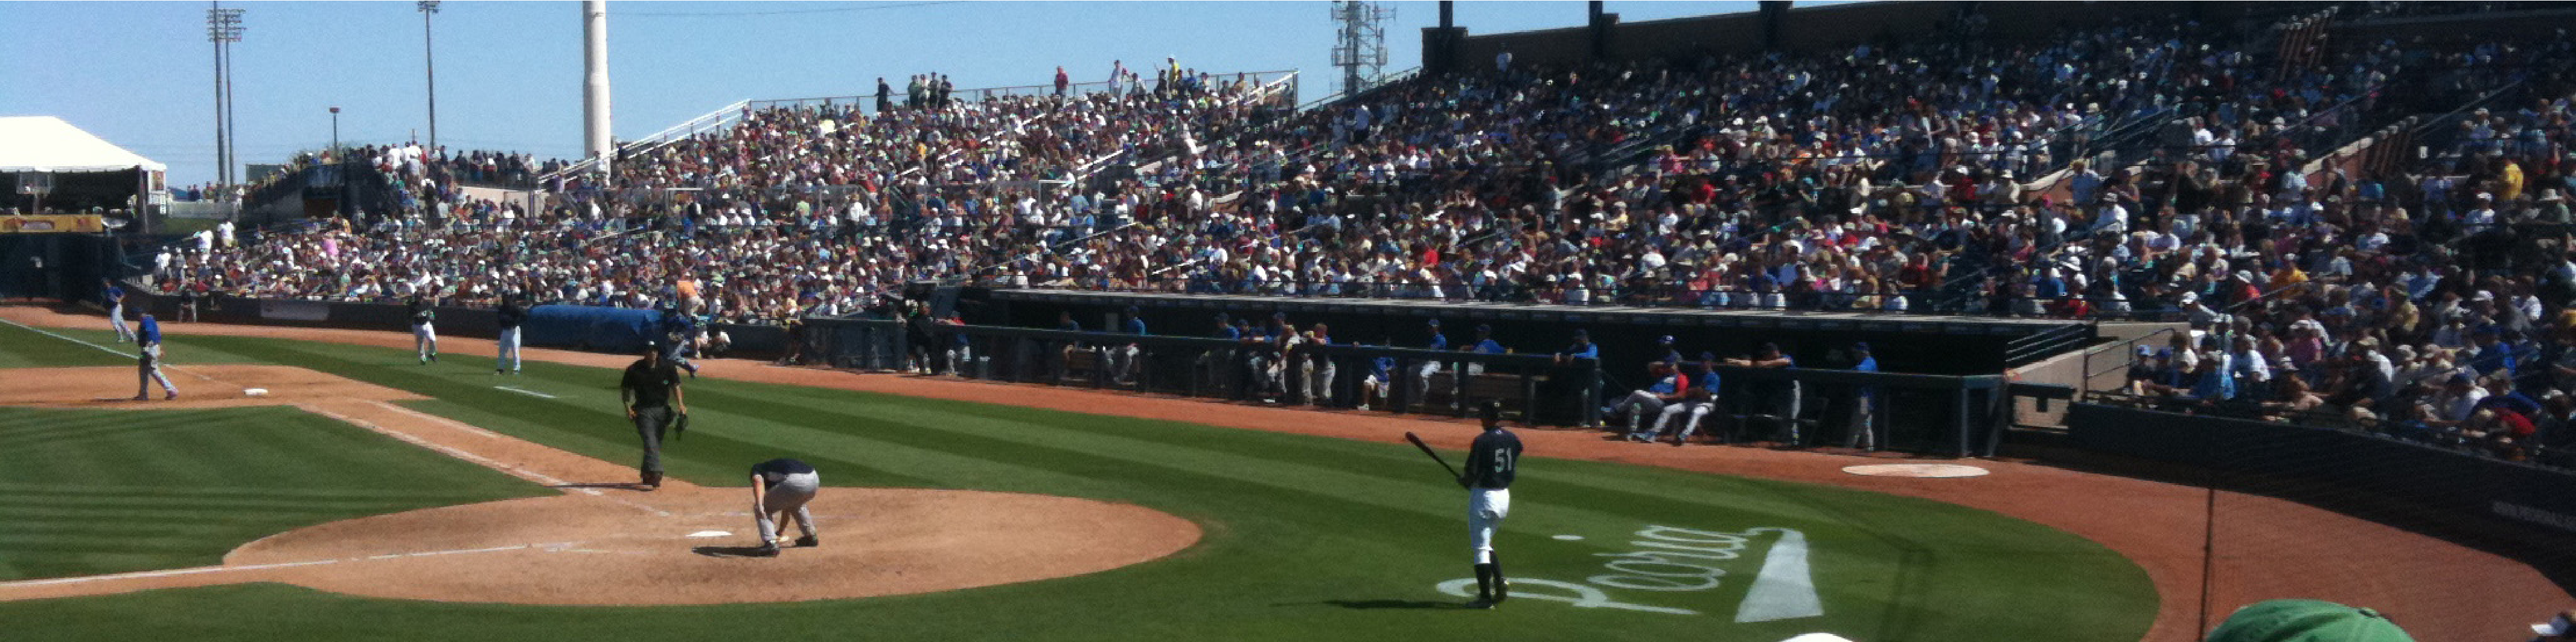
\includegraphics[width=\textwidth]{sampleteaser}
%   \caption{This is a teaser}
%   \label{fig:teaser}
% \end{teaserfigure}

\maketitle

\section{Introduction}
\label{introduction}

Recent  proliferation  of  Internet  technology  in
every  day's life  has  created  streaming  sources  that 
generate  data continuously, these data stream may comes from  a
variety of sources - social networks, on-line businesses, 
sensors,military surveillance to name a few. In the stream 
situation, data could not keep static steady (e.g. a data 
warehouse), so unlike traditional datasets, the stream of data 
flow into a computer system continuously and with varying 
arrival rates. They are time stamped, fast changing, massive, 
and potentially infinite. So current database could not store an 
entire data stream because of its tremendous volume. Therefore 
relative mining or analysis algorithms must process the data in 
real time and update the parameters decision boundaries as the 
stream progresses. 

Regression analysis is a widely  used  technique  for  the 
modeling and analysis of the relationship   between dependent 
variables and independent variables\cite{Friedman}.  In  the  
recent years, many research focus on applying regression 
analysis techniques to model and predict the behavior of the 
stream data. In this environment, main task for regression is 
learning a function of several input at-tributes from the past 
stream data with the goal of estimating as accurately as 
possible the value of a numerical target attribute in the future 
stream data \cite{Gama} \cite{Lughofer}. It is commonly assumed, 
in various ways, that the labeled source data available to train 
the linear regression model (pairs of input vectors and output 
scalars) is representative of the target data that it will use 
for making predictions (given only input vectors). Specifically, 
in real world, non-stationary  data generation process may 
induce arbitrary changes in data distribution over time.  In the 
previous times, a plethora  of  studies  have  proposed 
techniques to address these challenges. In the  
Gama\cite{Gama_drift} 's research, he proposed (); and 
Bifet\cite{Bifet} also proposed sliding windows to address the 
shift problem, their window size could be recomputed on-line 
according to the rate of change observed from the data in the 
window itself. However,these techniques  make  two  strong  
assumptions  about  the ability of applications employing them. 
In the previous papers , they often assume that true labels of 
data instances along the stream will be available soon after 
prediction, which is the first assumption. However, in the real 
world, true labels are  obtained using manual labeling mechanism 
under most of the situations, so it mat not occur as soon as 
possible. The another assumption is that  sample  data  
distribution of the training and test mini-batches are assumed 
to be equal during classification, this assumption may often be 
violated in many real-world applications. In this case, a 
mechanism to choose data instances  for  labeling  may  be  biased, this  induces  a  difference  in  data  distribution  between  the  training  and test data.  A regression model trained on a biased training dataset may perform poorly on future unbiased test data occurring along the stream. This is known as data drift \cite{Gama_drift}.
More specifically, data drift is a relationship between the target and source data distributions, such that $P_{tar}(y \vert {x}) = P_{src}(y \vert {x})$, and $P_{tar}(x) \ne P_{src}(x)$, here $x$ and $y$ denote the set of feature values and labels of the data instance respectively.



Except for the data shift, there is also another challenge 
called concept drift\cite{Parker}, which  occurs  in  a  stream  when  the  underlying concept of data changes over time. So, the  regression model needs  to  be  updated  regularly to adapt  to  the  most  recent concept. The  vast  majority  of  concept  drift  researches assume  that  true  labels  of  test instances  will  be  readily  available  to  update  the  classifier  as 
soon  as  they  are  tested.  However,  typically  labeling  
requires annotation  by  a  human  expert,  which  is  a  costly  and  time consuming process. More often, true labels are available only for a limited amount of data. Therefore, their  assumption suffer in this scenario.


  
  There are not so many effective methods which address regression algorithm under the data shift environment, recently, some people use the "re-weight" method. This method introduces strong inductive biases that are highly extrapolative, in recently, some improved method is proposed. In the paper\cite{chen}, the author established a robust bias-aware regression to solve the previous covariate shift problem that embraces the uncertainty resulting.Their approach assumes that the stochastic mapping from inputs to the output variable is as similar as possible to a "zero-knowledge" reference distribution, then they using minimax relative log-loss optimization approach to minimize relative loss in the worst case, and reduces to minimizing conditional Kullback-Leibler divergence. Comparing with a range of existing regression models on both synthetically created and natural bias datasets, their experiment's error value(also log-loss rate) performed best. However, this approach' s assume scenario did not include the concept drift occurs. What's more, their data stream only consist of single stream, not multi-stream,
  
  In  this  paper,  we  introduce  a  new  problem  setting  consisting of different types of data streams over the same domain, such that these assumptions can be relaxed.  A stream of labeled data instances are generated by a non-stationary process from a particular domain.  This is referred to as source stream.   Another  stream  of  data  instances  is  assumed  to be generated by an independent non-stationary process, referred to as target stream, from the same domain.
  
  
  Here are major contributions of this paper:
  
  1. We introduce a new data stream regression setting consisting of two independent non-stationary streams. The predicted value over target stream, using the data instances from source stream. We term this problem as Multi-stream Regression. 
  
  2. We design a covariate shift aware regression to address challenges in adapting the source data stream distribution, which may be biased, towards the target data stream distribution in a non-stationary environment. 
  
  3. We perform concept drift detection without requiring true dependent variable from the target stream, and using dependent variable observed on the source stream. 
  
  4. We evaluate this proposed approach empirically over several datasets, and compare the results with baseline method. The baseline method, Robust bias-aware regression, is come from the paper\cite{chen}

\section{Relative work}
\label{notations}
In this section, we present a brief discussion on covariate shift adaptation, concept drift and multistream regression. We also discuss some of the related work in this area.

\subsection{Covariate Shift Adaptation}
\label{notations}
In the fundamental data mining situation, people assume that both the training and test data represent
the same data distribution, known as the "stationary
distribution assumption". In the previous statement, we described that this assumption may be violated in real-world application. Addressing an arbitrary difference between training and test distribution is a very difficult problem\cite{Huang}. Hence, most approaches assume that the source and target data distributions $P_{src}(\cdot)$ and $P_{tar}(\cdot)$ are related through a covariate shift assumption. As the previous describe, the relationship
between the source and target data distributions is such that $P_{src}(y \vert {x}) = P_{tar}(y \vert {x})$ and $P_{src}(x) \ne P_{tar}(x)$,where x and y denote the
set of covariate values and label of the data instance respectively.

Recent studies focus on developing correction mechanisms for covariate shift, in the 
paper\cite{Huang}, Kernel Mean Matching (KMM) is proposed. In their algorithm, 
covariate shift between training and test data distributions is accounted by 
computing an importance weight $\beta(\textit{\textbf{x}}) = \frac{P_{tar}({x})}
{P_{src}({x})}$ . For each source instance x, we could use this algorithm in the 
learning process. Except for KMM algorithm, KLIEP\cite{sugiyama},and unconstrained

Least Square Importance Fitting (uLSIF)\cite{kanamori}, are among the techniques that 
are available in the literature for handling covariate shift in data. However, these 
approaches work only on fixed-size training and test data. For stream data, Kawahara 
and Sugiyama\cite{kawahara} extended previous KLIEP for direct online density ratio 
estimation and get good result. But this works on a single stream of data, where set 
of source/reference and target data instances are determined by a sliding window. In 
our paper, we consider multiple streams of data, where new data instance may arrive 
arbitrarily at any stream.


\subsection{Concept Drift}
\label{notations}
  Concept drift refers to scenario when the relation between input data $X$, e.g.,feature values, and the target variable $y$,e.g.,the labels will be changed over time. Formally, concept drift between time $t_0$ and $t_1$ can be defined as

\begin{equation}
   \exists X: p_{t0}(X,{y}) \ne p_{t1}(X,{y})
\end{equation} 

Where $p_{t0}(X,{y})$ represented the joint distribution between the set of input 
variables $X$ and the target label $y$ at time $t_{0}$, the same meaning for the 
variable $p_{t1}(X,{y})$ which happened at time $t_{1}$\cite{gama_survey}.The  
components of this equation include the prior probabilities of the labels
$p_{y}$, the class conditional probabilities $P(X \vert {y})$, distribution of incoming data $p_{X}$, and  the  posterior  probabilities  of  classes $P(y \vert 
{x})$. Real concept drift refers  to  the  changes  in  posterior  probabilities $P(y \vert {x})$. It may happen for several reasons including changes  in  incoming  data $p_{X}$.
  
  




\subsection{Multiple Stream Regression}
\label{statement}

Data stream regression is a challenging task due to its  inherent properties, e.g., 
infinite length, concept drift, etc.Infinite length problem is addressed by dividing 
the whole stream into fixed-size mini-batches. However, previous  works  suggesting for  mining/regression  data  stream are  typically  based  on  the  single  data stream model. Recently, a few works have mentioned or addressed the multiple  data  streams (MDS) model  and  some  related  issues Recent approaches mostly concentrate on multiple stream research. Although the research on multiple data streams (implicitly or explicitly) not started for a long time, the  model of multiple  data  streams  has been involved  in  most  of  the recent  data  stream  applications, such as advances  in  micro-electro-mechanical  system, wireless  communication  technology and so on.

  From  the  above introduction,  multiple data stream are  different  from the  single stream model in the following aspects.The first aspect is multiple data stream has many domain data sources to generate distributed data streams independently. What's more, there are requirements over all  the  data  streams  (such as comparing the  local  pattern  vs. the regional/global  pattern,  and synchronizing data points  from  these  data  streams). At last, it  is difficult  or  impractical  to  simply  view  and  treat  the  data  from different  data  sources  as  a  single  data  stream  with  multiple marginal probability, this means that source and target data 
represent the same data distribution.
  
  Here a new problem setting, proposed, called Multistream Regression, in this situation, two data streams over the same domain are considered relaxing the following assumptions:  first, true labels of data instances along the stream would not available soon after prediction, because true labels are often associated with human effort,time, and other resources. Second, with previous statement, it is assumed while regression that source and target data represent the different data distribution.
  
 


\section{PRELIMINARIES}
\label{notations}
In this section, we formalize the multistream regression problem and present challenges of performing  regression over drifting data streams in this context
Through out this paper, we are using the notations mentioned in 
the above table to describe concepts of the data stream. 
Consider there is a process that generating continuous stream of 
data instances from a domain $D$. Also, a data instance is
denoted as $(x, y)$, where $x$ is composed of a vector of $m$ in
${D^{m}}$, and $y$ is the corresponding value for each data
instances. Suppose there are two processes $S$ and $T$ in
the domain of $D$ to represent the source and target data stream.
In process $S$, values of both $x$ and $y$ are available, while
in process $T$, only value of $x$ is available. Thus, a 
$Multistream Regression$ problem can be defined as follows:

Suppose $X_{s}$ is a set of n-dimensional vectors of variables
and $Y_{s}$ is the corresponding actual value of a source data 
stream in a certain domain $D$. Meanwhile, $X_{t}$ is a set of 
n-dimensional vectors of variables in a target data stream in the
same domain. We want to build a regression model $f_{ens}$ to
estimate the value that corresponds $X_{T}$ using $X_{s}$,
$Y_{s}$ and $X_{T}$.

\ref{tab1}.

\begin{table}[H]
\centering
\caption{Notations}
\label{tab1}
\begin{tabular}{|l|l|}
\hline
 Symbol & Meaning \\ \hline
 $D$ & Domain \\ \hline
 $x$ & Independent variables of $m$ dimensions \\ \hline
 $y$ & Value of a data instance \\ \hline
 $S$ & Source data stream with actual $y$ \\ \hline
 $T$ & Target data stream without actual $y$  \\ \hline
 $M$ & Parameter matrix of regression model  \\ \hline
 $f_{src}$ & Probability distribution function of source data \\ \hline 
 $f_{tgt}$ & Probability distribution function of target data \\ \hline
 $f_{ens}$ & Ensemble of regression model \\ \hline
 $f_{tm}$ & Probability distribution of target mini batch \\ \hline
\end{tabular}
\end{table}



\subsection{Challenges}
\label{challenges}
Normally we assume that inputs in the source set follow the
same distribution as the inputs in the target set, so that
source
data would provide solid information in predicting instances in
the target set. However, this assumption is not always valid in 
a multistream setting. Equivalently, consider sample
probability distributions of $S$ and $T$ within a certain time period.
$P_{S}^{t}(y|x) = P_{T}^{t}(y|x)$ and $P_{S}^{t}(x) \neq P_{T}^{t}
(x)$ at time $t$. In this condition, the distribution of $P(x)$ is biased 
in source compared to that in target, and this condition is called 
$covariate shift$.

Meanwhile, in a real time regression analysis setting such as
predictions to data stream, there is another challenge normally
referred as $concept drift$. It means that due to the nature
that pattern of data can evolve over time, that is, the
conditional probability distribution may change over time in the target stream. Specifically in our problem at time $t$,
$P_{S}^{t}(y|x) \neq P_{T}^{t}(y|x)$. In this paper, we assume
that two data streams with in the same domain $D$ will have
synchronous data drifts, which can be seen in Figure
\ref{fig:multistream}.



% \begin{figure}
% \centering
% 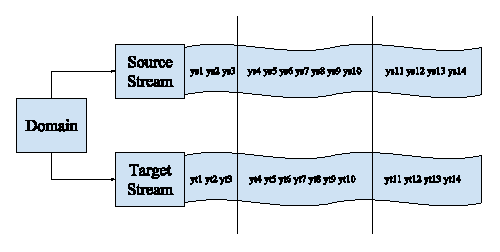
\includegraphics{fig_multistream.eps}
% \caption{Demonstration of synchronous data covariate shifts on data streams}
% \label{fig:multistream}
% \end{figure}

Predictions for computational problems about data stream is 
increasingly
important over recent years. Many scholars had been exploring 
topic within
this area, such as theory, databases and networks.(babcock1, 
estan1,
Muthukrishanan1)

\section{Multistream Regression}

% here I generate the pseudocode for multistream regression
\makeatletter
\def\BState{\State\hskip-\ALG@thistlm}
\makeatother

\begin{algorithm}
\caption{Multistream Regression}\label{driftdetection}
\begin{algorithmic}[1]
\Procedure{detectDrift}{}
\BState \textbf{begin}:
\State $B_s$, $B_t$ $\gets$ \textit{readData}$(S,T,I)$
\State $E_{param} \gets \textit{buildModel} (B_s, B_t)$
\While {$S$ or $T$ $exists$}
\State $B_s, B_t \gets readData(S,T,1)$
\State $W_s \gets getError(E_{param}, B_s)$
\State $W_t, \hat{Y} \gets preData(E_{param}, B_t)$
\If {$z \gets checkDrift(W_s)$}
\State $B_s, W_s \gets updateBuffer$$(z, B_s, W_s)$
\State $E_{param} \gets buildSourceModel(B_s)$
\EndIf
\State $\hat{y} \gets getPrediction(E_{param}, B_{t})$
\State print $getAccuracy (\hat{y}_t, B_t)$
\EndWhile
\EndProcedure
\end{algorithmic}
\end{algorithm}

\subsection{Initialization and Covariate Shift Correction}
Basically, a conditional logloss on the target distribution is considered to follow the equation:
\begin{equation*}
	logloss_{f_{tgt}(x)}(f(y|x), \hat{f}(y|x)) = E_{f_{tgt}(x)f(y|x)}[-log\hat{f}(Y|X)] % need change here
\end{equation*}

Here this conditional logloss is an evaluator of the level of
covariate shift by measuring the "surprise" to tell samples from
$f_{tgt}(x)f(y|x)$ while actually is from $f_{tgt}(x)\hat{f}
(y|x)$ \cite{Lafferty01}.Thus, if there isn't significant 
covariate shift from the target set to the source set, the
solution could be a minimax robust estimation approach subject to
quadratic squares solution to regression. After all the
regression estimator should be the one that is robust to the the
data set that has most covariate shift inside.
\begin{equation} \label{eq1}
\begin{split}
\mu \left( x, M \right) = \left( 2\frac { f_{ src }\left( x \right)  }{ f_{ tgt }\left( x \right)  } M_{ (y,y) }+\frac { 1 }{ { \sigma  }^{ 2 } } { \mu  }_{ 0 } \right)^{-1} \\ 
  \left( -2\frac { f_{ src }\left( x \right)  }{ f_{ tgt }\left( x \right)  } M_{ y,x1 }\left[ \begin{matrix} x \\ 1 \end{matrix} \right] +\frac { 1 }{ { \sigma  }^{ 2 } } { \mu  }_{ 0 } \right)
\end{split}
\end{equation}

In this paper, we store our source data ($S$) and target data ($T$) in a data buffer framework, and we can refer these two as $B_{S}$ and $B_{T}$. These two buffers are the initial conditions to train our ensemble model $E$. 



\subsection{Value Prediction}
Now we can use the matrix derived in Section \ref{challenges} to
predict the value for every instance in the dataset. This
prediction is based on the Minimax estimation formulation, and
it minimizes the target distribution conditional
$Kullback-Leiber$ divergence. Hence the Covariate Shift problem
is addressed by this algorithm. Also, the logloss is evaluated
via the $getLogloss$ function in Algorithm 1. Now we have the confident
that data in both source and target dataset are unbiased.


\subsection{Drift Detection}

In this section, a $detectDrift$ method is introduced to label those 
points in a data stream where significant changes happen.These
changes are referred as concept drift.
We can use the generated $\hat{y}$ in the target set, along
with those instances with $y$ in the source set, to figure out 
the drift point although the stream. 
A concept drift along $S$ could significantly impact the performance of
Multistream regression model. Here, the concept drift we mentioned
here specifically indicates a $within-stream$ drift. This type
of concept drift can cause change in the data distribution. Once
the change point is detect, the problem could be handled by
training another regression model so that the regression
parameters can be updated. We would expect the prediction accuracy would be greatly improved once we mark the drift points and update the regression model accordingly.

\subsubsection{Window Management}
In order to detect the change point accurately, two
sliding windows on both source stream and target stream are
maintained. The reason to do this is that we want to generate
feedback on most recent data.
The predicted value of data instances is generated by the
regression model, and is inserted into $W_t$. In the window,
there is ensemble confidence score resulting from regression of
data instances of $T$. Then values of confidence are generated 
within a range of [0,1]. Based on the nature of the confidence
level, where the confidence is usually high in value until there 
is a concept drift, here we apply a $beta$ distribution to model the
confidence level. Note here that the window management schema for source 
stream is to follow the corresponding window in the target stream, so 
that most recent data can be used for training purposes if there is a 
concept drift in the stream.

\subsubsection{Change Detection}
We propose a change point detection method to check for
significant change in the $T$, the target stream. The reason of 
existence of window management



\makeatletter
\def\BState{\State\hskip-\ALG@thistlm}
\makeatother



\begin{algorithm}
\caption{Concept Drift detection}\label{driftdetection}
\begin{algorithmic}[1]
\Procedure{detectDrift}{}
\BState \textbf{begin}:
\State \textit{Threshold} $\gets$ $-log({\alpha}_d)$, $n$ $\gets$ size of $W_h$, and $\omega_n$ $\gets$ 0
\If {$n \leq S_{max}$ $\&$ $mean(W_h[1:n] > 0.5$} 
\For {$q \gets \gamma$ : $n - \gamma$}
\State Estimate pre and post change distribution 
\State parameters, $\theta_{\alpha}$ and $\theta_{\beta}$ from $W_x[1:q]$ and 
\State $W_h[q+1:n]$ respectively
\State Calculate $s(q,n)$ using Equation (3)
\EndFor
\State $\omega_{n} = \max_{\gamma \leq q \leq n-\gamma}s(q,n)$
\If {$\omega_n \geq Threshold$}
\State \Return false
\Else
\State \Return -1
\EndIf
\Else
\State \Return 0
\EndIf
\EndProcedure
\end{algorithmic}
\end{algorithm}
        

\subsection{Drift Adaption}
\label{driftadaption}
As we mentioned before, parameters generated by the regression
model will be updated once a concept drift is detected. 

\section{Experiment}
\subsection{Datasets}
In this paper, we use 3 synthetic datasets for evaluation
purposes. All information of these 3 datasets are listed in the table below
For these dataset, we introduce biased source in each dataset, followed by a method used in previous studies.

\begin{table}[H]
\centering
\caption{Dataset}
\label{tab2}
\begin{tabular}{|l|l|l|}
\hline
 \bf{Dataset} & \bf{No. of features} & \bf{No. of instances} \\ \hline
 $globalAbrupt$ & 5 & 10,000\\ \hline
 $globalGradual$ & 5 & 10,000\\ \hline
 $localAbrupt$ & 5 & 10,000\\ \hline
\end{tabular}
\end{table}



\subsection{Experiments}



\subsubsection{Baseline Method}

As we mentioned before, there are methods that handles covariate shift in the
dataset well but not concept drift in the multistream setting.
In this paper, we use those methods as our baseline methods. Thus the advantages of applying concept drift detection and adaption method can be observed. This model used in the paper are called robust regression (robRegression).

\begin{figure*}
\centering
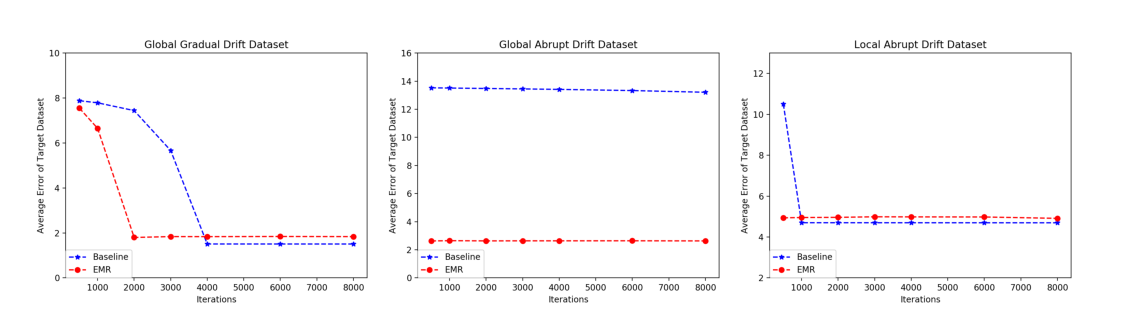
\includegraphics{fig_iterationview.eps}
\caption{Iteration: MAE on three datasets}
\label{fig:iterationview}
\end{figure*}

\subsection{Results}

\newenvironment{figurehere}
{\def\@captype{table}}
{}


\begin{table}[H]
\centering
\caption{Increasing Iteration}
\label{tab2}
\begin{tabular}{|l|l|l|l|l|l|l|}
\hline
          & \multicolumn{2}{l|}{globalAbrupt} & \multicolumn{2}{l|}{globalGradual} & \multicolumn{2}{l|}{localAbrupt} \\ \hline
Iteration & Baseline        & EMR             & Baseline         & EMR             & Baseline        & EMR            \\ \hline
500       & 13.52     & 2.62     & 7.88      & 7.55     & 10.50     & 4.93    \\ \hline
1000      & 13.50     & 2.64     & 7.78      & 6.65     & 4.69     & 4.95    \\ \hline
2000      & 13.47     & 2.63     & 7.44      & 1.79     & 4.69     & 4.96    \\ \hline
3000      & 13.44     & 2.63     & 5.66      & 1.83     & 4.69     & 4.98    \\ \hline
4000      & 13.41     & 2.63     & 1.50      & 1.83     & 4.69     & 4.98    \\ \hline
6000      & 13.32     & 2.63     & 1.50      & 1.84     & 4.69     & 4.97    \\ \hline
8000      & 13.20     & 2.63     & 1.50      & 1.83     & 4.69     & 4.91    \\ \hline
\end{tabular}
\end{table}

Figure\ref{fig:iterationview} demonstrate progress we made by our Efficient Multistream
Regression method. We evaluates the prediction accuracy using
Mean Absolute Error (MAE). Two approaches demonstrated in these figures are
the baseline approach, and our EMR approach. From the figure, we can see that the
prediction accuracy converges over the iterations trained in each
section. For the dataset with Global Abrupt Drift, the EMR method
outperforms the baseline method for every iterations. And, we can
tell that EMR performs
better compared to the baseline method in every dataset
significantly. 

\begin{figure*}
\centering
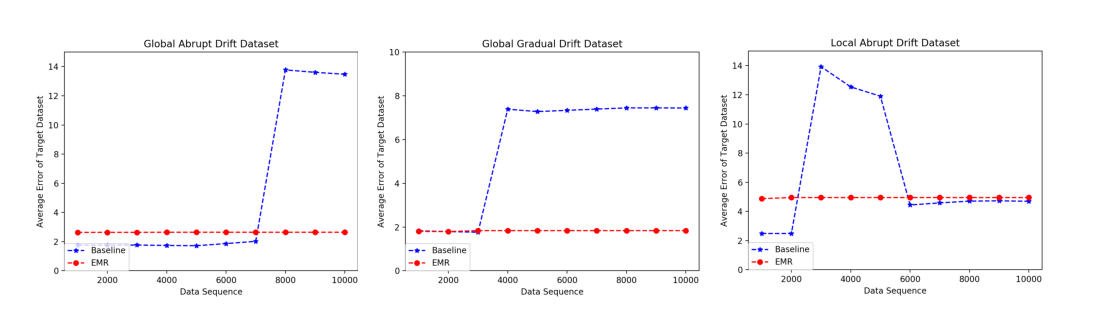
\includegraphics{fig_streamview.eps}
\caption{Stream: MAE on three datasets}
\label{fig:streamview}
\end{figure*}

\begin{table}[H]
\centering
\caption{Stream: MAE on three datasets}
\label{tab2}
\begin{tabular}{|l|l|l|l|l|l|l|}
\hline
          & \multicolumn{2}{l|}{globalAbrupt} & \multicolumn{2}{l|}{globalGradual} & \multicolumn{2}{l|}{localAbrupt} \\ \hline
Instance & Baseline        & EMR             & Baseline         & EMR             & Baseline        & EMR            \\ \hline
1000       & 1.75     & 2.63     & 1.82      & 1.79     & 2.48     & 4.87    \\ \hline
2000      & 1.75     & 2.63     & 1.79      & 1.79     & 2.48     & 4.95    \\ \hline
3000      & 1.76     & 2.63     & 1.76      & 1.83     & 13.92     & 4.95    \\ \hline
4000      & 1.73     & 2.64     & 7.38      & 1.83     & 12.54     & 4.95    \\ \hline
5000      & 1.71     & 2.64     & 7.27      & 1.83     & 11.90     & 4.95    \\ \hline
6000      & 1.86     & 2.64     & 7.33      & 1.83     & 4.44     & 4.95    \\ \hline
7000      & 2.01     & 2.64     & 7.39      & 1.83     & 4.58     & 4.95    \\ \hline
8000      & 13.77     & 2.64     & 7.44      & 1.83     & 4.70     & 4.95    \\ \hline
9000      & 13.16     & 2.64     & 7.44      & 1.83     & 4.72     & 4.95    \\ \hline
10000      & 13.47     & 2.64     & 7.44      & 1.83     & 4.69     & 4.95    \\ \hline

\end{tabular}
\end{table}

\section{Conclusion and future work}
\label{conclusion}

In this paper, we propose a efficient multistream regression
framework to address the prediction problem regarding two data
streams - source and target.
Generally speaking true value of dependent variable is only
available in a source stream ($Y_s$), and is used to make
predictions of dependent variable on a target stream along with
independent variables on both streams ($X_s$ and $X_t$). 
Challenges of addressing problems of having covariate shift and
concept drift simultaneously in two data streams is widely
discussed. Our solution involves a minimax approach for
regressions under covariate shift, and concept drift
detection techniques to correct drift. Following experiments
shows that our solution had generated much better performance in
terms of prediction accuracy on various of datasets, compared to
the baseline model.

There are some future work that we can think of to extend the use
of the proposed framework in this paper. For example, in this
paper we assume that concept drift happens
simultaneously in both source and target data stream. However,
these data drifts can occur asynchronously as well. Hence there
is opportunities to discuss the effect of asynchronous drift on the prediction accuracy as well.

\appendix
%Appendix A

\section{References}
Generated by bibtex from your \texttt{.bib} file.  Run latex,
then bibtex, then latex twice (to resolve references)
to create the \texttt{.bbl} file.  Insert that \texttt{.bbl}
file into the \texttt{.tex} source file and comment out
the command \texttt{{\char'134}thebibliography}.
% This next section command marks the start of
% Appendix B, and does not continue the present hierarchy
\section{More Help for the Hardy}

Of course, reading the source code is always useful.  The file
\path{acmart.pdf} contains both the user guide and the commented
code.

% \begin{acks}
%   The authors would like to thank Dr. Yuhua Li for providing the
%   matlab code of  the \textit{BEPS} method. 

%   The authors would also like to thank the anonymous referees for
%   their valuable comments and helpful suggestions. The work is
%   supported by the \grantsponsor{GS501100001809}{National Natural
%     Science Foundation of
%     China}{http://dx.doi.org/10.13039/501100001809} under Grant
%   No.:~\grantnum{GS501100001809}{61273304}
%   and~\grantnum[http://www.nnsf.cn/youngscientsts]{GS501100001809}{Young
%     Scientsts' Support Program}.

% \end{acks}


\bibliographystyle{ACM-Reference-Format}
\bibliography{sigproc} 

\end{document}
